\documentclass[10pt,utf8]{beamer}

\mode<presentation> {
%  \usetheme{Boadilla}
  \usetheme{Madrid}
%	\usetheme{Fzu}
  \setbeamercovered{transparent}
}

\usepackage{palatino}
\usepackage{graphicx}
\usepackage{array}
\usepackage{color}
\usepackage{subfigure}
\usepackage{colortbl}
\usepackage{amsmath}
\usepackage{hyperref}
\usepackage{listings}
\usepackage{fancyvrb}
\usepackage[export]{adjustbox}
%\usepackage{tikz}
%\usetikzlibrary{arrows,shapes,backgrounds}


\definecolor{MyDarkGreen}{rgb}{0.3,0.7,0.3}

\setbeamertemplate{caption}{\raggedright\insertcaption\par} %turn off caption prefix ("Figure")

\title{Introduction to Infinispan}
\author{Vojtěch Juránek}
\institute[Red Hat]{JBoss - a division by Red Hat}
\date{21.~3.~2016, FI MUNI, Brno}

\newenvironment{mylisting}
{\begin{list}{}{\setlength{\leftmargin}{1em}}\item\scriptsize\bfseries}
{\end{list}}

\newenvironment{mytinylisting}
{\begin{list}{}{\setlength{\leftmargin}{1em}}\item\tiny\bfseries}
{\end{list}}

% see http://tex.stackexchange.com/questions/151254/coloring-or-bolding-multiple-lines-in-fancyvrb-integration-with-listings
\lstdefinestyle{Java}{
	basicstyle          = \small\ttfamily,
	language            = Java,
	numbers             = left,
	numberstyle         = \tiny,
	stepnumber          = 1,
	numbersep           = 5pt,
	backgroundcolor     = \color{white},
	showspaces          = false,
	showstringspaces    = false,
	showtabs            = false,
	frame               = single,
	tabsize             = 2,
	captionpos          = b,
	breaklines          = true,
	breakatwhitespace   = false,
	morestring          = [b]",
	stringstyle         = \color{blue},
	keywordstyle        = \color{magenta},
	commentstyle        = \color{gray},
	identifierstyle     = \color{black},
	moredelim           = **[is][\bfseries]{`}{`},
	moredelim           = **[is][\color{magenta}]{|}{|}, %Scala style not available, mark keyworkds by hand
  moredelim           = **[is][\color{gray}]{!}{!}, %Scala style not available, mark keyworkds by hand
	fancyvrb            = true,
}
\lstdefinestyle{Bash}{
	basicstyle          = \small\ttfamily,
	language            = Bash,
	numbers             = left,
	numberstyle         = \tiny,
	stepnumber          = 1,
	numbersep           = 5pt,
	backgroundcolor     = \color{white},
	showspaces          = false,
	showstringspaces    = false,
	showtabs            = false,
	frame               = single,
	tabsize             = 2,
	captionpos          = b,
	breaklines          = true,
	breakatwhitespace   = false,
	morestring          = [b]",
	stringstyle         = \color{blue},
	keywordstyle        = \color{magenta},
	commentstyle        = \color{gray},
	identifierstyle     = \color{black},
	moredelim           = **[is][\bfseries]{`}{`},
	moredelim           = **[is][\color{magenta}]{|}{|}, 
	fancyvrb            = true,
}
\lstdefinestyle{Protobuf}{
	basicstyle          = \scriptsize\ttfamily,
	language            = Bash,
	numbers             = left,
	numberstyle         = \tiny,
	stepnumber          = 1,
	numbersep           = 5pt,
	backgroundcolor     = \color{white},
	showspaces          = false,
	showstringspaces    = false,
	showtabs            = false,
	frame               = single,
	tabsize             = 2,
	captionpos          = b,
	breaklines          = true,
	breakatwhitespace   = false,
	morestring          = [b]",
	stringstyle         = \color{blue},
	keywordstyle        = \color{magenta},
	commentstyle        = \color{gray},
	identifierstyle     = \color{black},
	moredelim           = **[is][\bfseries]{`}{`},
	moredelim           = **[is][\color{magenta}]{|}{|}, 
	fancyvrb            = true,
}

\begin{document}

%\tikzstyle{every picture}+=[remember picture]
%\tikzstyle{na} = [baseline=-.5ex]


\begin{frame}
 \titlepage
\end{frame}

\begin{frame}
	\frametitle{Course materials download}
	\scriptsize{
	\begin{itemize}
		\item Course materials, including this presentation:\\
		\color{blue}\url{https://developer.jboss.org/wiki/AdvancedJavaEELabFIMUNIJaro2016}\color{black}
		\item or slightly update presentation:\\ 
		\color{blue}\url{https://github.com/vjuranek/presentations/tree/master/CTU_Prague2016}\color{black}
	\end{itemize}
	}
\end{frame}

\begin{frame}
	\centering
	\huge{\textbf{Data today}}
\end{frame}


\begin{frame}
	\frametitle{Data today}
	\begin{figure}
		\centering
		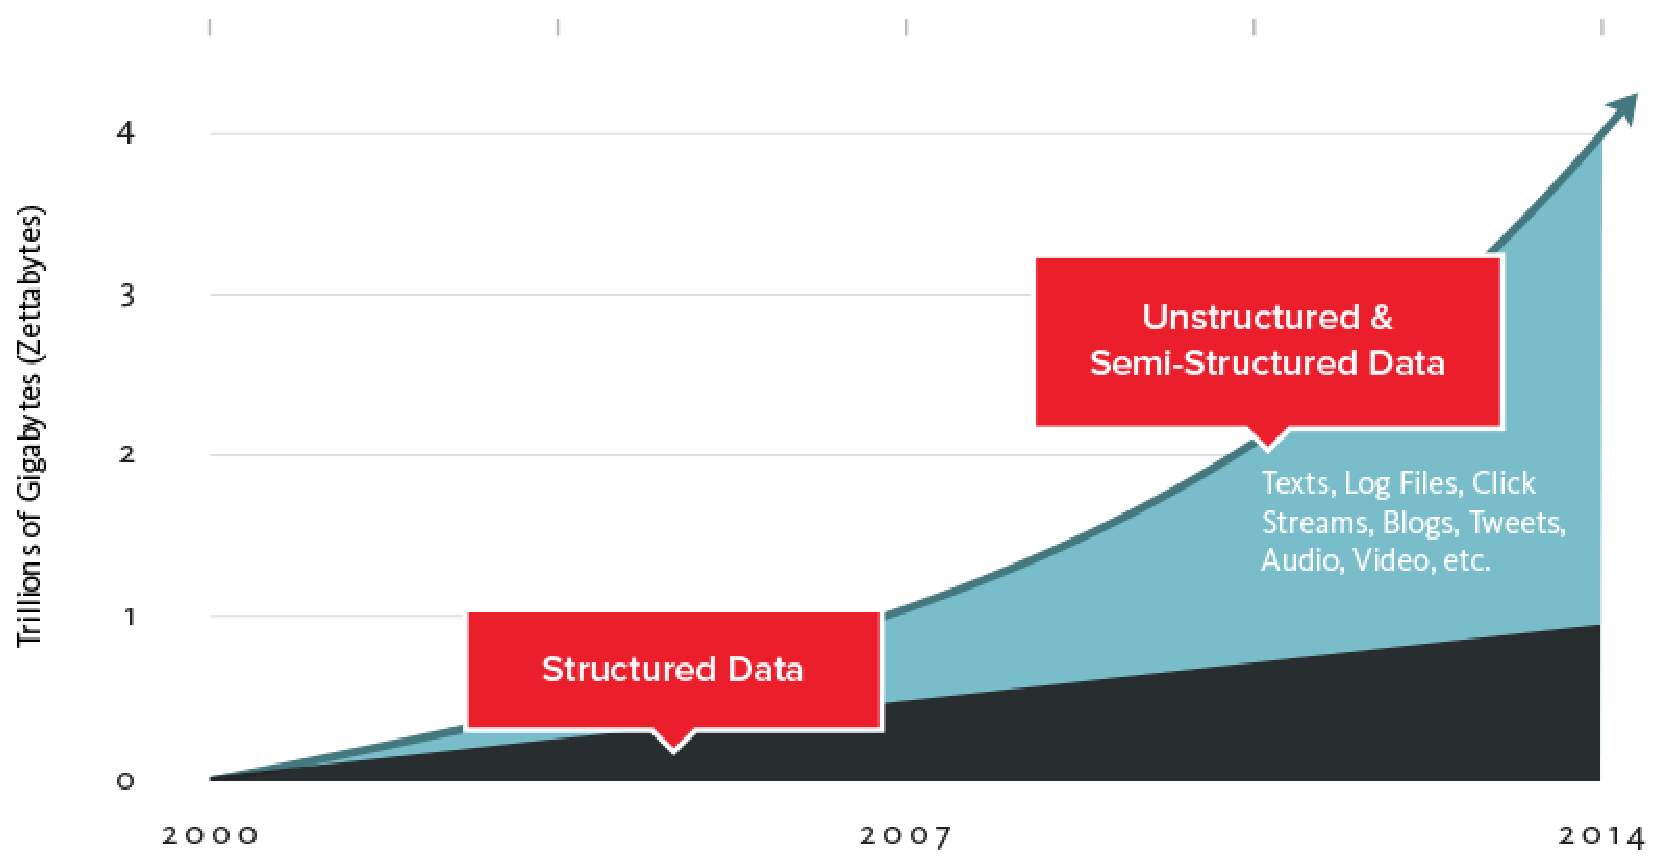
\includegraphics[width=10cm]{./img/why-nosql-2.eps}
		\caption{\tiny{Source: \url{http://www.couchbase.com/nosql-resources/what-is-no-sql}}}
	\end{figure}
\end{frame}

\begin{frame}
	\frametitle{How big are Big data?}
	\visible<2,3> {
		\begin{figure}
			\centering
			
\includegraphics[width=8cm]{./img/borat_big_data.eps}
			\caption{\tiny{Source: \url{https://twitter.com/DEVOPS\_BORAT/status/288698056470315008}}}
		\end{figure}
	}
	\visible<3> {
		\begin{itemize}
			\item Data collection so large and complex it's impossible to process it on one computer
			\item You can scale up, but sooner or later you'll have to scale out
		\end{itemize}
	}
\end{frame}

\begin{frame}
	\frametitle{Big data characteristics}
	%\href{https://en.wikipedia.org/wiki/Big\_data#Characteristics}{wikipedia} says:
	\begin{itemize}
		\pause
		\item \textbf{Volume:} unprecedented amount of data being stored
		\pause
		\item \textbf{Velocity:} speed at which the data is generated
		\pause
		\item \textbf{Variety:} the type and nature of the data - from structured data in traditional databases to unstructured text documents, email, video, audio etc.
		\pause
		\item \textbf{Variability:} the amount of incoming data can highly vary
		\pause
		\item \textbf{Veracity:} the quality of captured data can vary greatly as well
	\end{itemize}
\end{frame}

\begin{frame}
	\frametitle{Big data - some of the challenges}
		\begin{itemize}
			\item Analysis run on top of the huge amount of data
			\item Ability to store huge amount of unstructured data (often for performance reasons)
			\item But also ability  to talk to RDBMS or query structured data is often needed as well
			\item Highly scalable solution (also because of cost effectiveness)
			\item Cloud architecture - everything is ephemeral
			\item Information privacy
		\end{itemize}
\end{frame}

\begin{frame}
	\frametitle{NoSQL}
	\visible<2> {
		\begin{figure}
			\centering
			
\includegraphics[width=10cm]{./img/borat_learn_nosql.eps}
			\caption{\tiny{Source: \url{https://twitter.com/devops_borat/status/141368065110708224}}}
		\end{figure}
	}
\end{frame}

\begin{frame}
	\frametitle{NoSQL}
	\begin{itemize}
		\item Nature of the data
		\pause
		\item More flexible data mode
		\pause
		\item Better scalablity
		\pause
		\item Performance
	\end{itemize}
	\begin{figure}
		\centering
		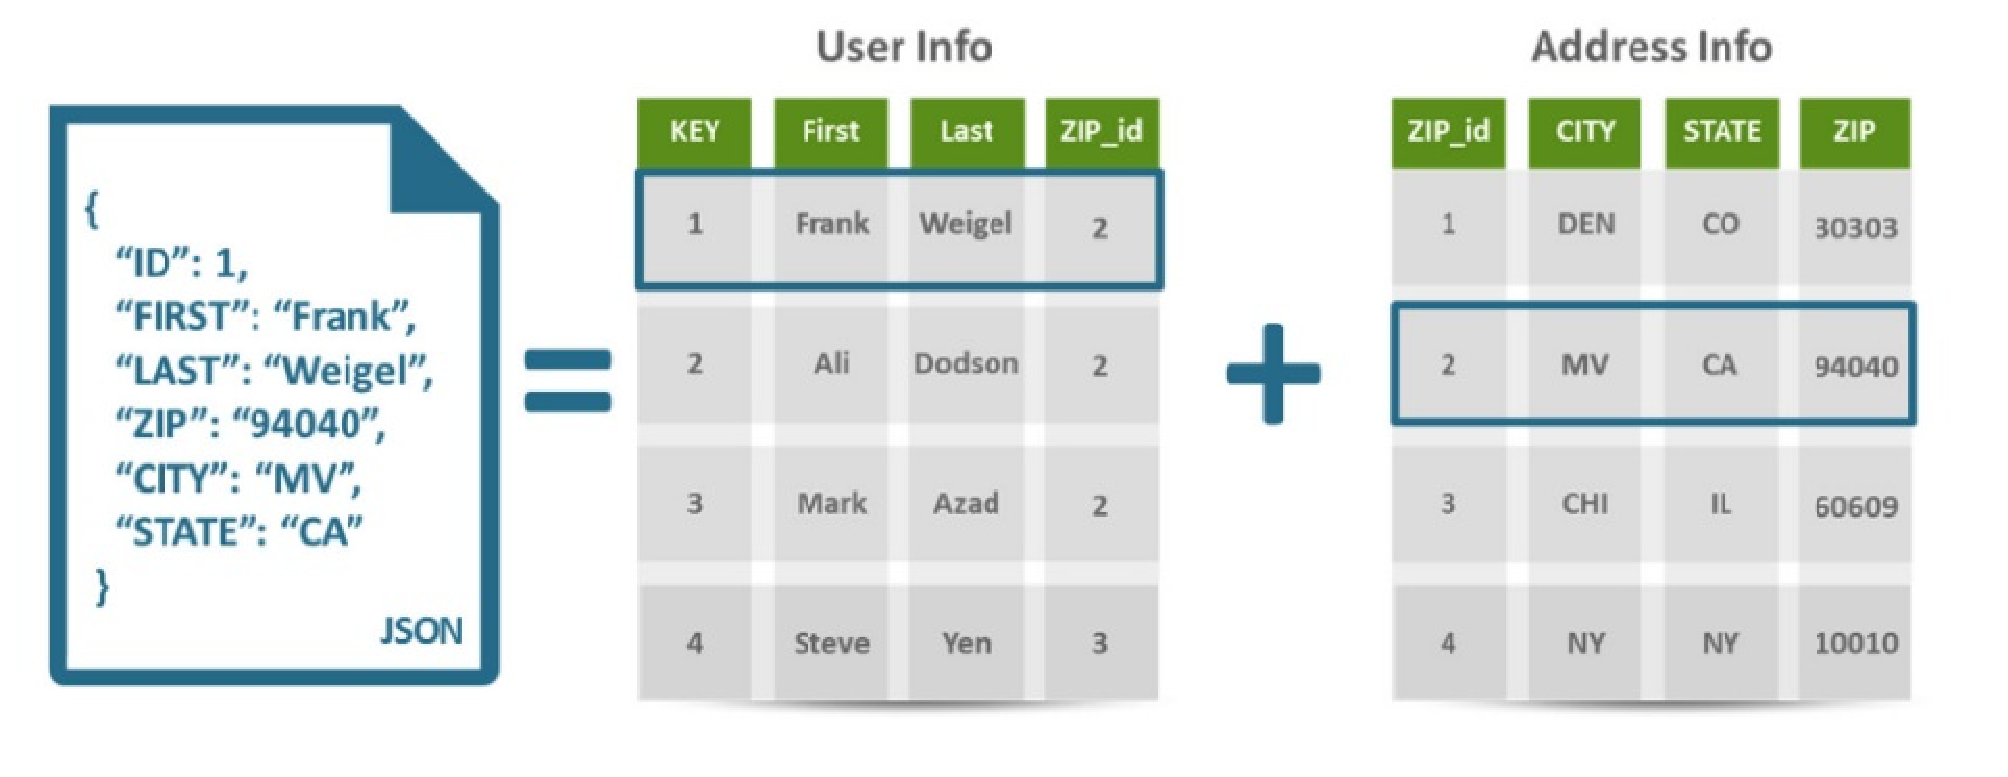
\includegraphics[width=10cm]{./img/json_vs_sql.eps}
		\caption{\tiny{Source: \url{www.couchbase.com/sites/default/files/uploads/all/whitepapers/NoSQL-Whitepaper.pdf}}}
	\end{figure}
\end{frame}

\begin{frame}
	\centering
	\huge{\textbf{What is a data grid?}}
\end{frame}

\begin{frame}
	\frametitle{What is a data grid?}
	\begin{itemize}
	 \item An in-memory distributed data store designed for fast access to large volumes of data and scalability.
	 \item Commonly a complementary layer to the relational database and the application.
	\end{itemize}
	\centering
	\visible<2> {
	\color{blue}\textbf{Key data grid characteristics:}\color{black}
	\begin{itemize}
	 \item In-memory, distributed caching
	 \item Elastic and scalable
	 \item Advanced querying
	 \item Data replication
	 \item Processing for streaming data
	 \item Transaction capabilities
	\end{itemize}
	}
\end{frame}

\begin{frame}
	\frametitle{Why in-memory}
	\begin{figure}
		\centering
		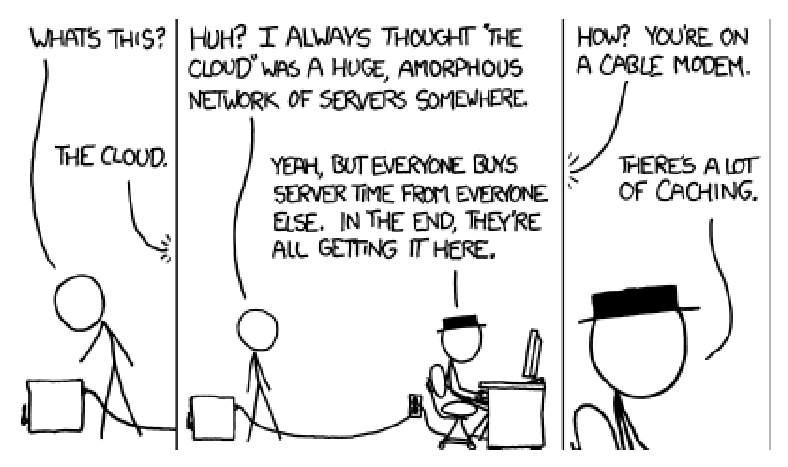
\includegraphics[width=12cm]{./img/xkcd_908.eps}
		\caption{\tiny{Source: Part of \href{http://xkcd.com/908/}{xkcd \#908}}}
	\end{figure}
\end{frame}

\begin{frame}
	\frametitle{Why in-memory}
	\begin{itemize}
	 \item Lots of data is needed in real-time (BigData $\rightarrow$ FastData)
	 \pause
	 \item Some tasks can be completed much faster when data are kept in memory
	 \pause
	 \item Keeping data in memory during processing of whole application stack, not only during processing in one application in the stack
	 \pause
	 \item With data replication you can keep your data only in memory (no need to store them in persistent storage)
	\end{itemize}
\end{frame}

\begin{frame}
	\frametitle{Scalability vs. elasticity}
	Sometimes used as synonyms, but usually
	\begin{itemize}
		\item \textbf{Scalability:} ability of the system to deal reasonable well with increasing load (data volume, traffic volume, complexity etc.), usually just by adding more resources.
		\item \textbf{Elasticity:} ability to fit the resources needed to cope with changed loads dynamically. Sometimes elasticity refers to fit the resources (add/remove resources) in an automated manner, when needed. 
	\end{itemize}
\end{frame}


\begin{frame}
	\centering
	\huge{\textbf{Infinispan}}
\end{frame}

\begin{frame}
	\frametitle{Infinispan}
	\begin{columns}
	\column{0.38\textwidth}
		\begin{figure}
			\centering
			
\includegraphics[width=3cm]{./img/infinispan.eps}
		\end{figure}
		\vspace{0.38cm}
		\color{blue}
			\url{https://infinispan.org}\\
			\vspace{0.1cm}
			\scriptsize{\url{https://github.com/infinispan}}\\
		\color{black}
		\scriptsize{(Apache License, v2.0)}
	\column{0.6\textwidth}
		\begin{itemize}
			\item In-memory data grid platform, written in Java
			\pause
			\item Schema-less (optionally), No-SQL key-value data store
			\pause
			\item Distributed cache - offers massive memory
			\pause
			\item Elastic and scalable - can run on hundreds of nodes
			\pause
			\item Highly available - no SPOF, resilient to node failures
			\pause
			\item Multi-version concurrency control (MVCC)
			\pause
			\item Transactional
			\pause
			\item Queryable
			\pause
			\item Processing for streaming data
		\end{itemize}
	\end{columns}
\end{frame}

\begin{frame}[fragile]
	\frametitle{Infinispan cache}
	\begin{itemize}
		\item Infinispan takes care about all that hard stuff.
		\item From user perspective Infinispan cache is \textbf{just a map!}
	\end{itemize}
	\vspace{0.3cm}
	\begin{lstlisting}[style=Java]
		DefaultCacheManager cacheManager = new DefaultCacheManager("my_ispn_config.xml");
		Cache<String, String> cache = cacheManager.getCache("myCache");
		cache.put("key", "value");
		String value = cache.get("key");
	\end{lstlisting}
\end{frame}

\begin{frame}
	\frametitle{Infinispan (embedded) high level architecture}
	\begin{figure}
		\centering
		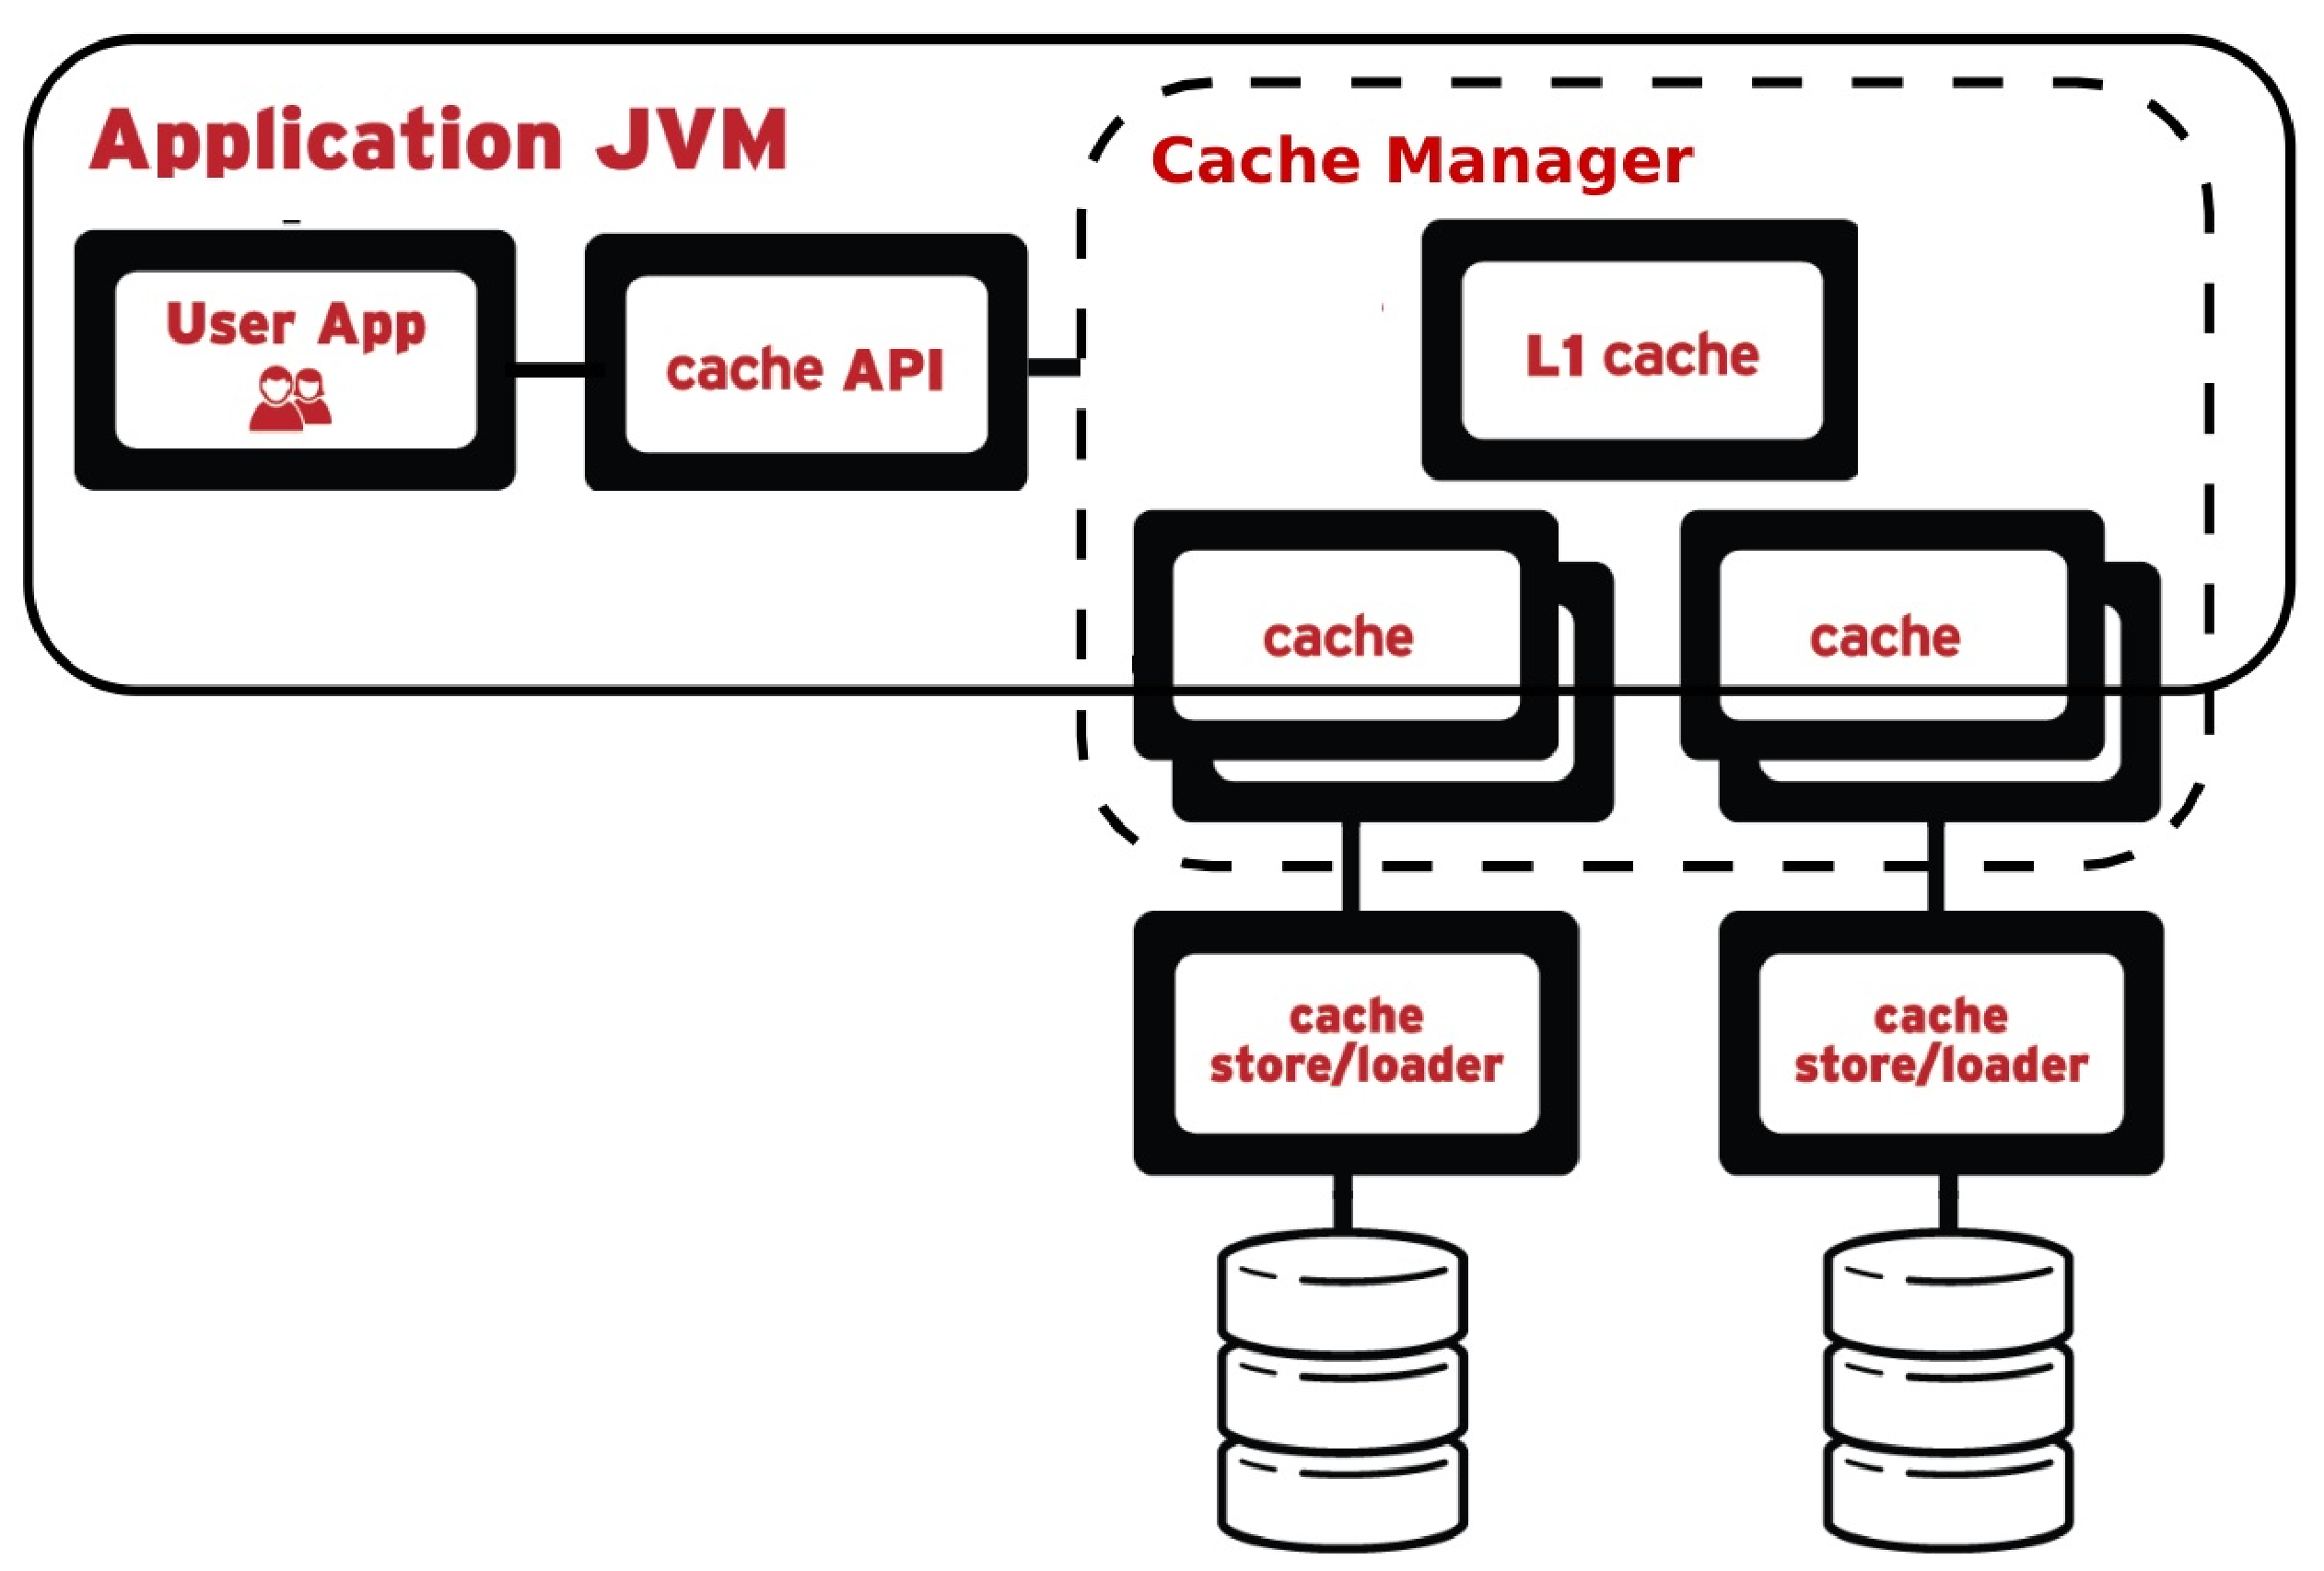
\includegraphics[width=10cm]{./img/ispn_high_level_emb.eps}
	\end{figure}
\end{frame}

\begin{frame}[fragile]
	\frametitle{Infinispan embedded tutorial}
	Simple weather app using embedded Infinispan
	\begin{itemize}
		\item \small{\url{http://infinispan.org/tutorials/embedded/}}
		\item \small{\url{https://github.com/infinispan/infinispan-embedded-tutorial}}
	\end{itemize}
	\vspace{0.3cm}
	\begin{lstlisting}[style=Bash]
		git clone https://github.com/infinispan/infinispan-embedded-tutorial.git
		cd infinispan-embedded-tutorial
		git checkout -f step-2
		sed -i 's/<!-- a/<a/;s/t -->/t>/' pom.xml #switch to local random weather service
		mvn clean package
		mvn exec:exec
	\end{lstlisting}
\end{frame}

\begin{frame}
	\frametitle{Commercial break: JGroups}
	\href{http://jgroups.org/}{\color{blue}\textbf{JGroups}} is a toolkit for reliable messaging written in Java. \\
	It can be used to create clusters whose nodes can send messages to each other.\\
	\vspace{0.5cm}
	\textbf{Main features:}
	\begin{itemize}
		\pause
		\item Cluster creation and deletion. Cluster nodes can be spread across LANs or WANs.
		\pause
		\item Membership detection and notification about joined/left/crashed cluster nodes.
		\pause
		\item Sending and receiving of node-to-cluster messages (point-to-multipoint).
		\pause
		\item Sending and receiving of node-to-node messages (point-to-point).
		\pause
		\item Detection and removal of crashed nodes.
	\end{itemize}
	More about JGroups in upcoming \textbf{WildFly clustering course}!
\end{frame}

\begin{frame}
	\frametitle{Clustering modes}
	\begin{itemize}
		\item Under the hood leverages JGroups project for clustering.
		\item Data is distributed and replicated in the background.
		\item Nodes can be added or removed smoothly.
	\end{itemize}
	\vspace{-0.1cm}
	
	\visible<2> {
	\begin{columns}
	\column{0.5\textwidth}
		\begin{itemize}
			\item Local - no clustering
			\vspace{2.9cm}
			\item Replicated
			\begin{figure}
				%\centering
				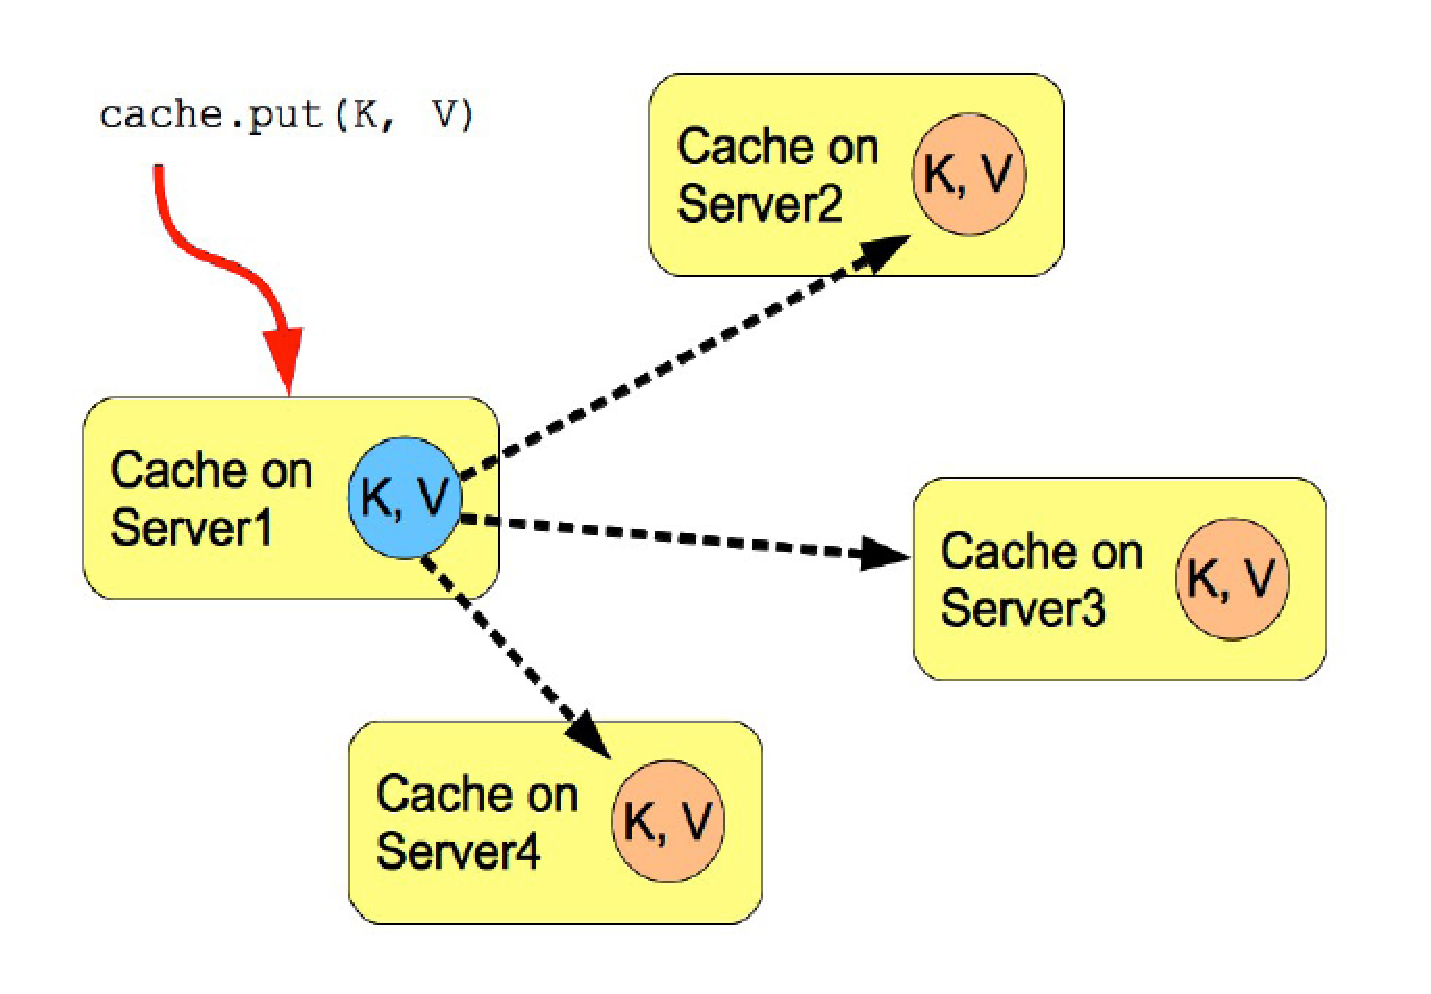
\includegraphics[width=4cm]{./img/ispn-repl.eps}
			\end{figure}
		\end{itemize}
	\column{0.5\textwidth}
		\begin{itemize}
			\item Invalidation
			\begin{figure}
				%\centering
				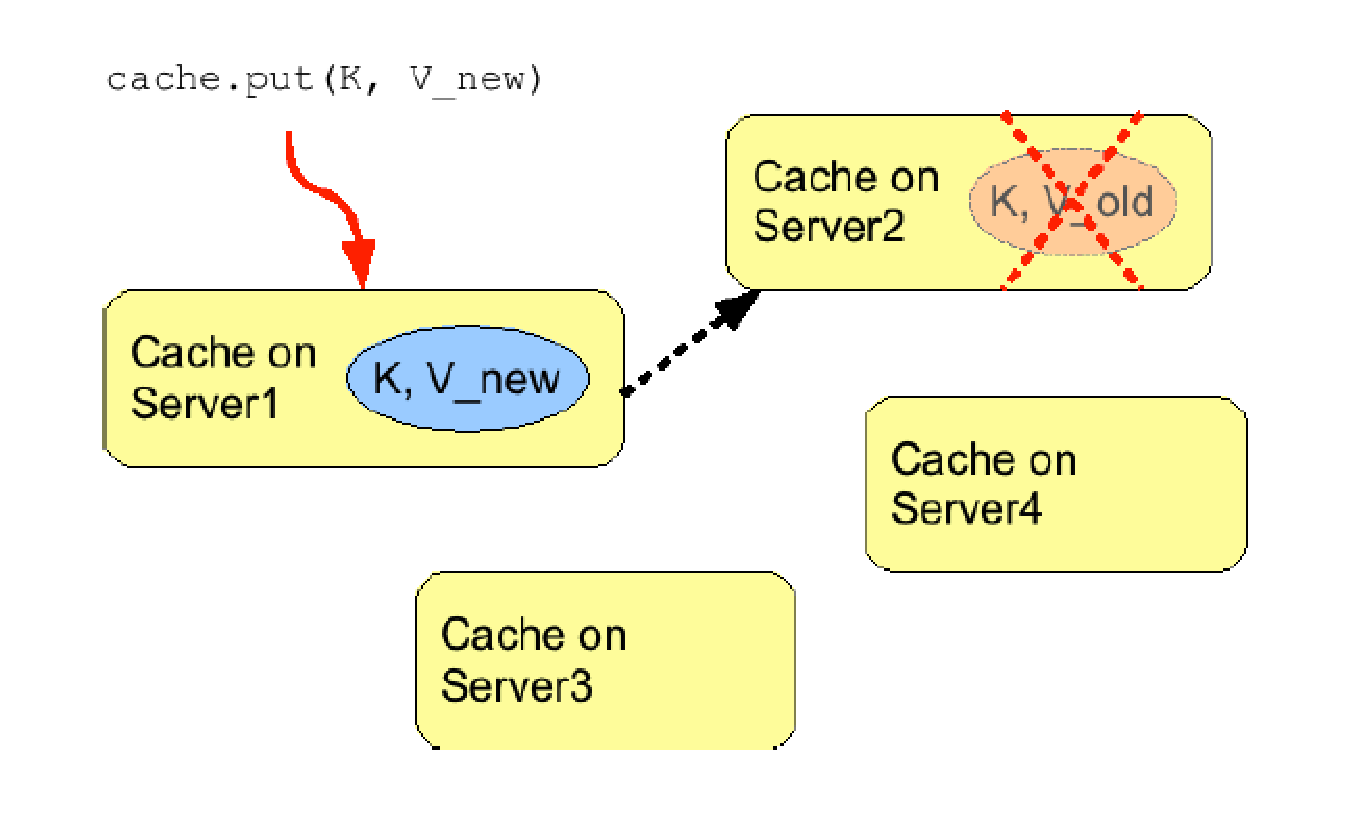
\includegraphics[width=4cm]{./img/ispn-inval.eps}
			\end{figure}
			\vspace{-0.1cm}
			\item Distributed
			\begin{figure}
				%\centering
				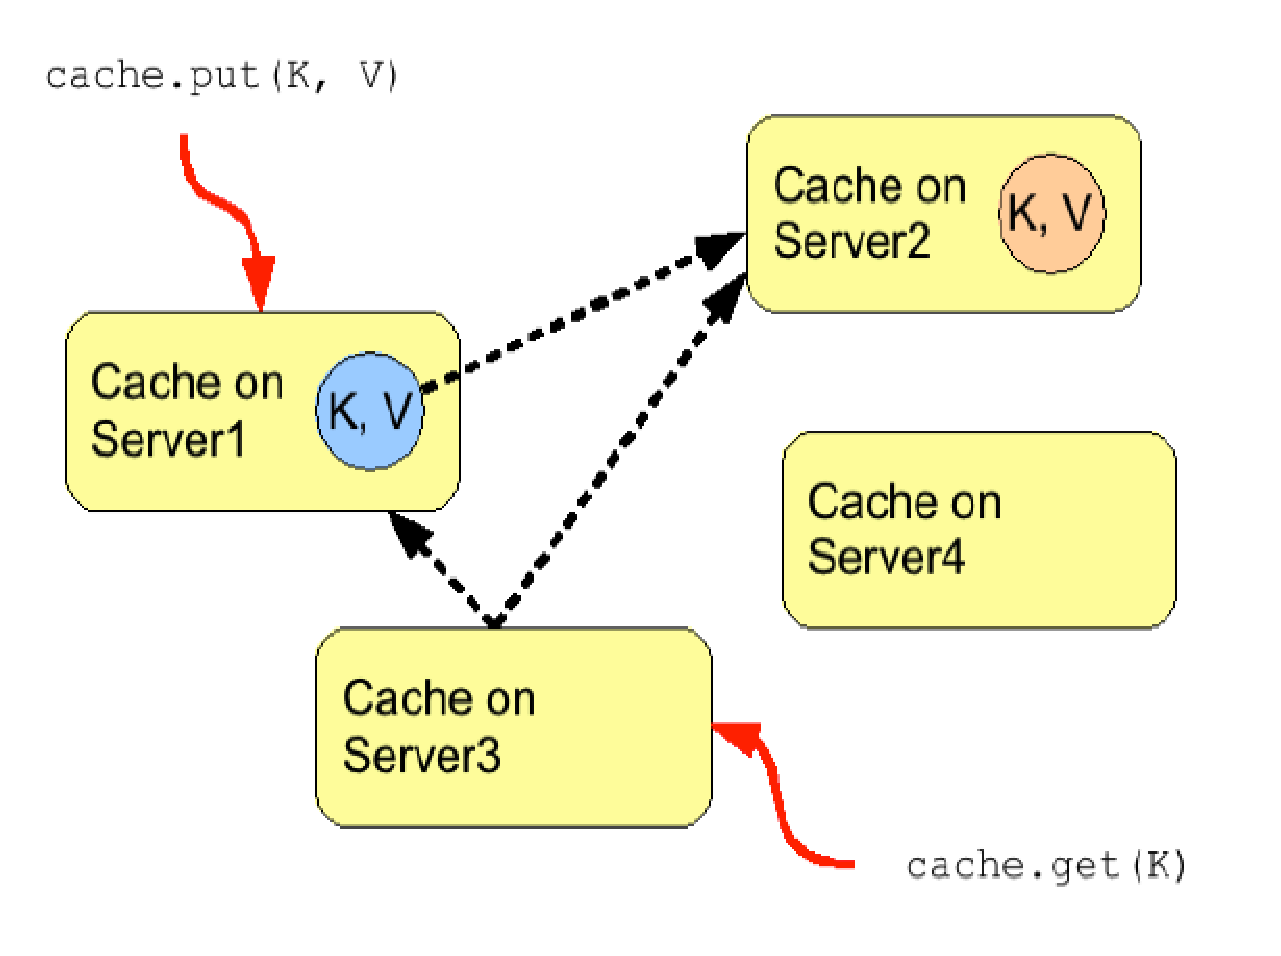
\includegraphics[width=4cm]{./img/ispn-dist.eps}
			\end{figure}
		\end{itemize}
	\end{columns}
	}
\end{frame}

\begin{frame}
	\frametitle{Infinispan modes}
	\begin{columns}
	\column{0.5\textwidth}
		\begin{itemize}
			\item Embedded (library, in-VM)
		\end{itemize}
		\begin{figure}
			%\centering
			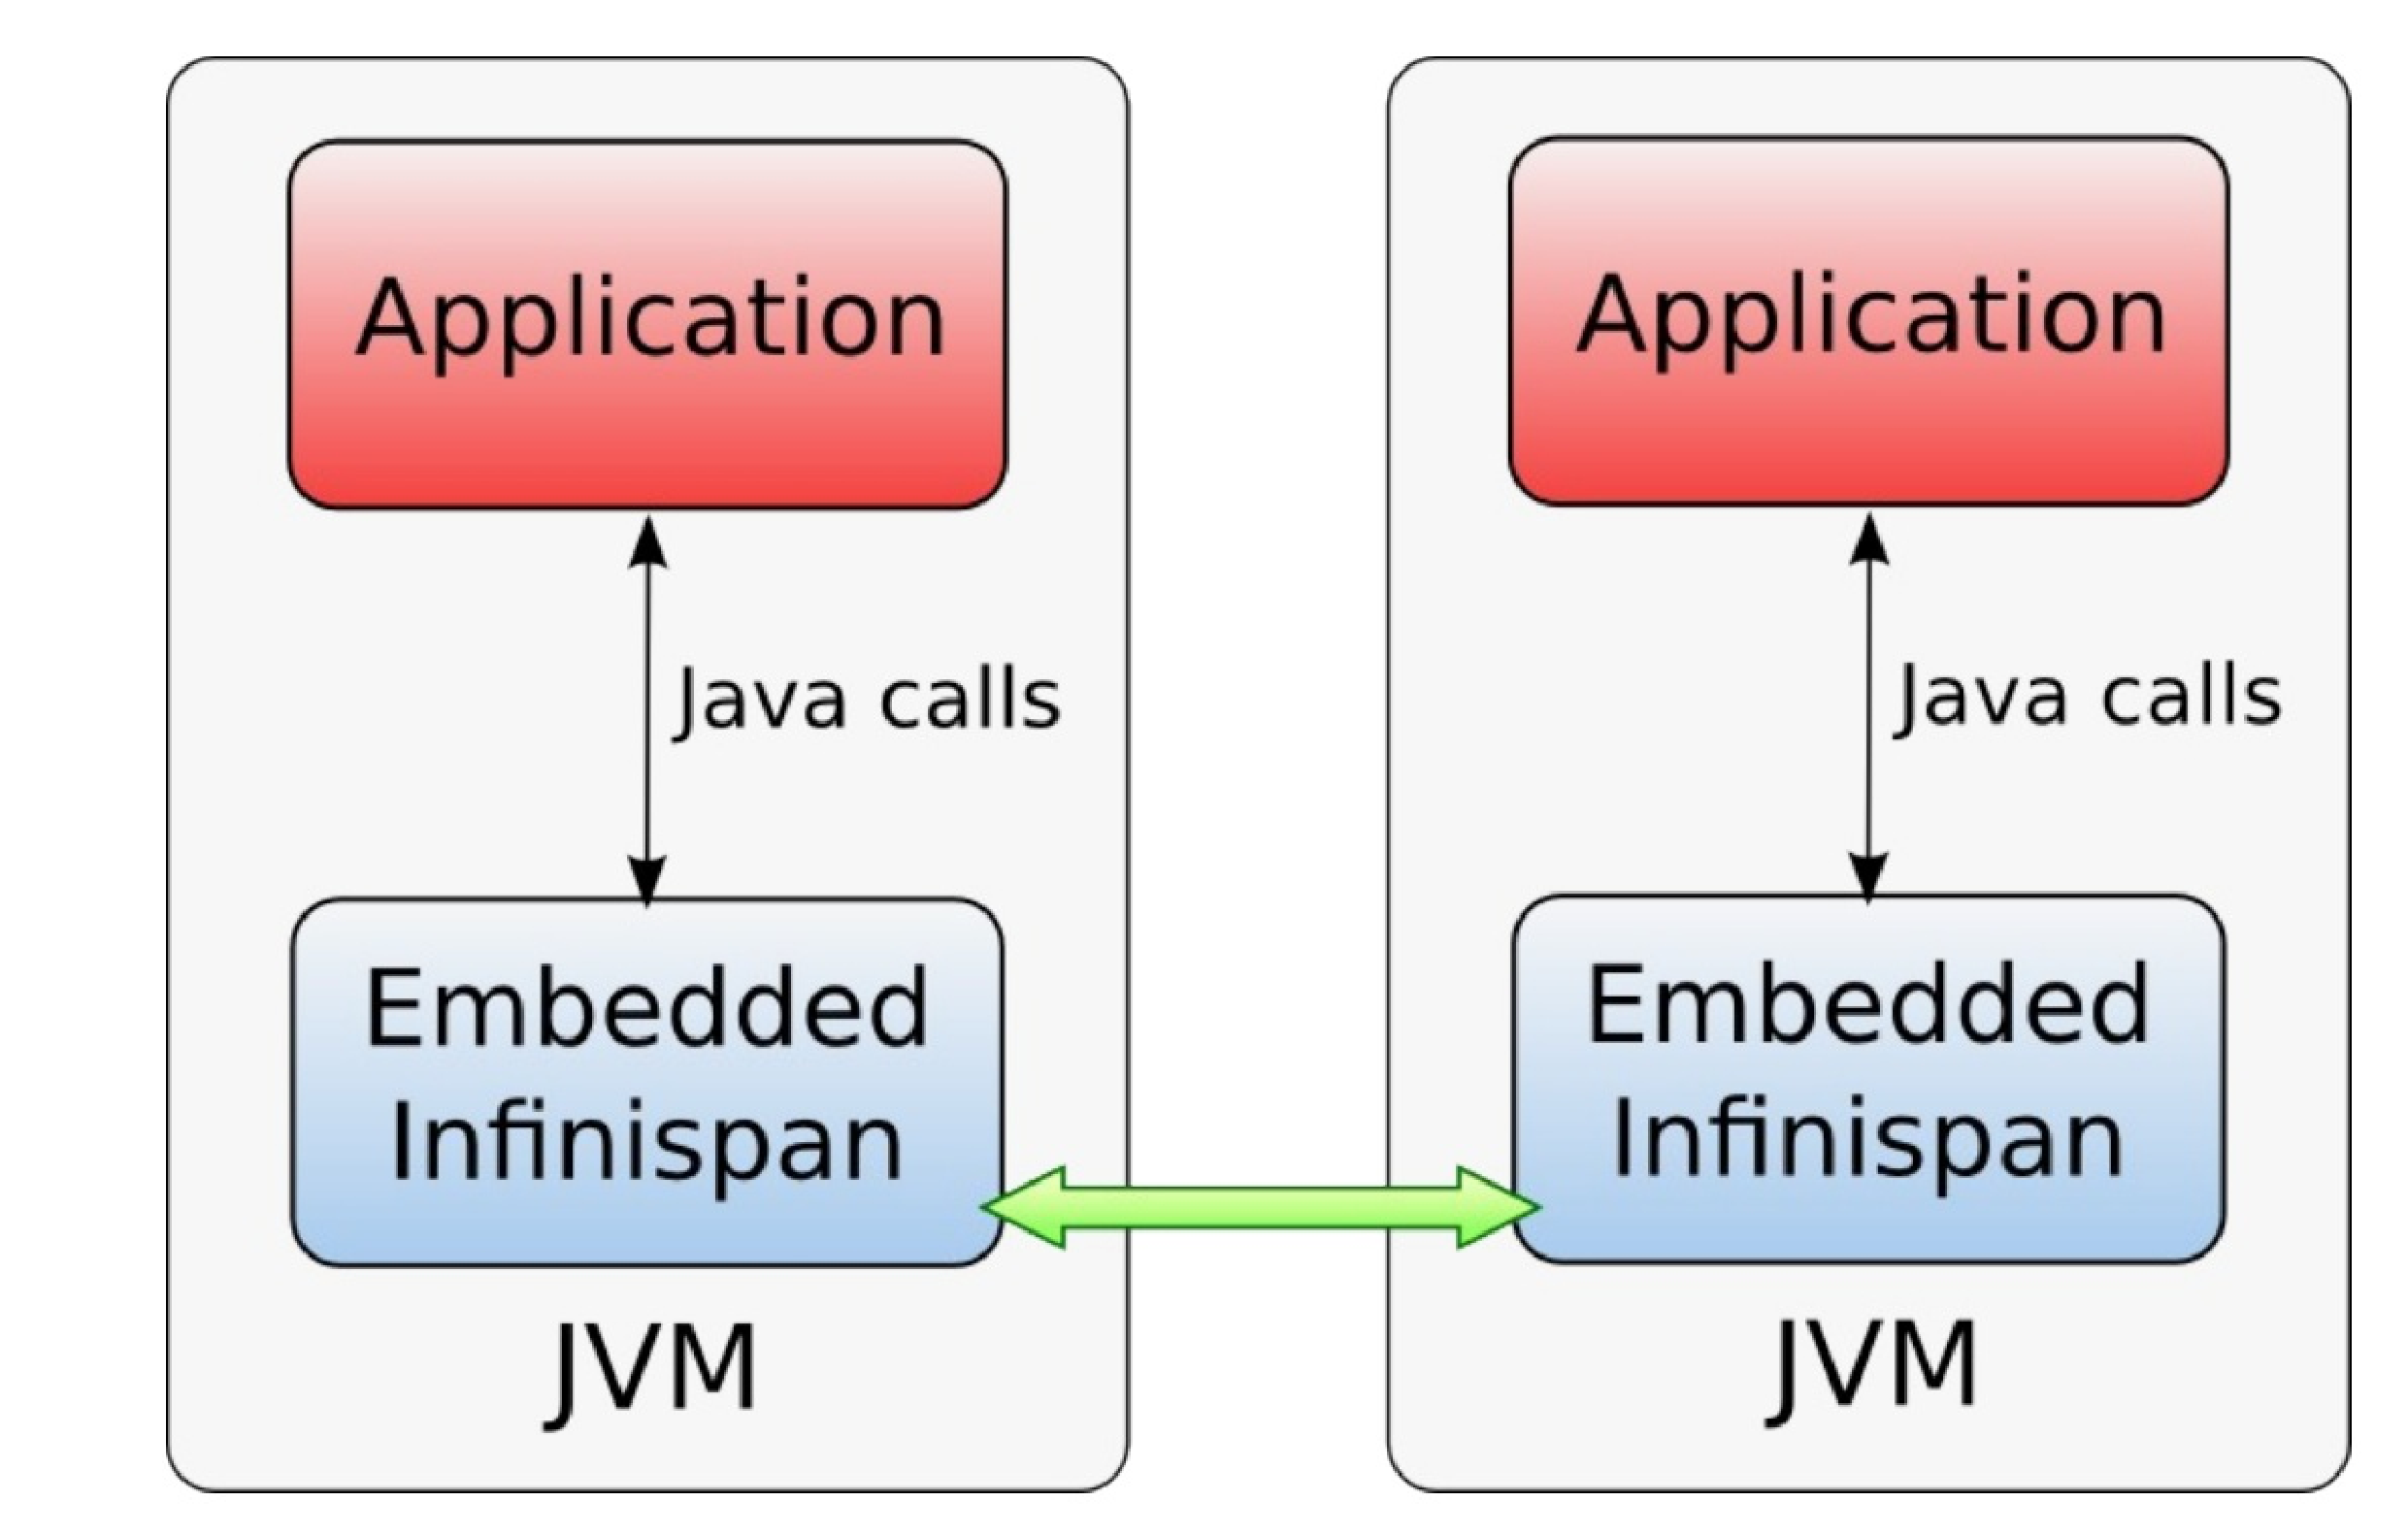
\includegraphics[width=5cm]{./img/ispn-emb.eps}
		\end{figure}
	\column{0.5\textwidth}
		\begin{itemize}
			\item Client-server (remote)
		\end{itemize}
		\begin{figure}
			%\centering
			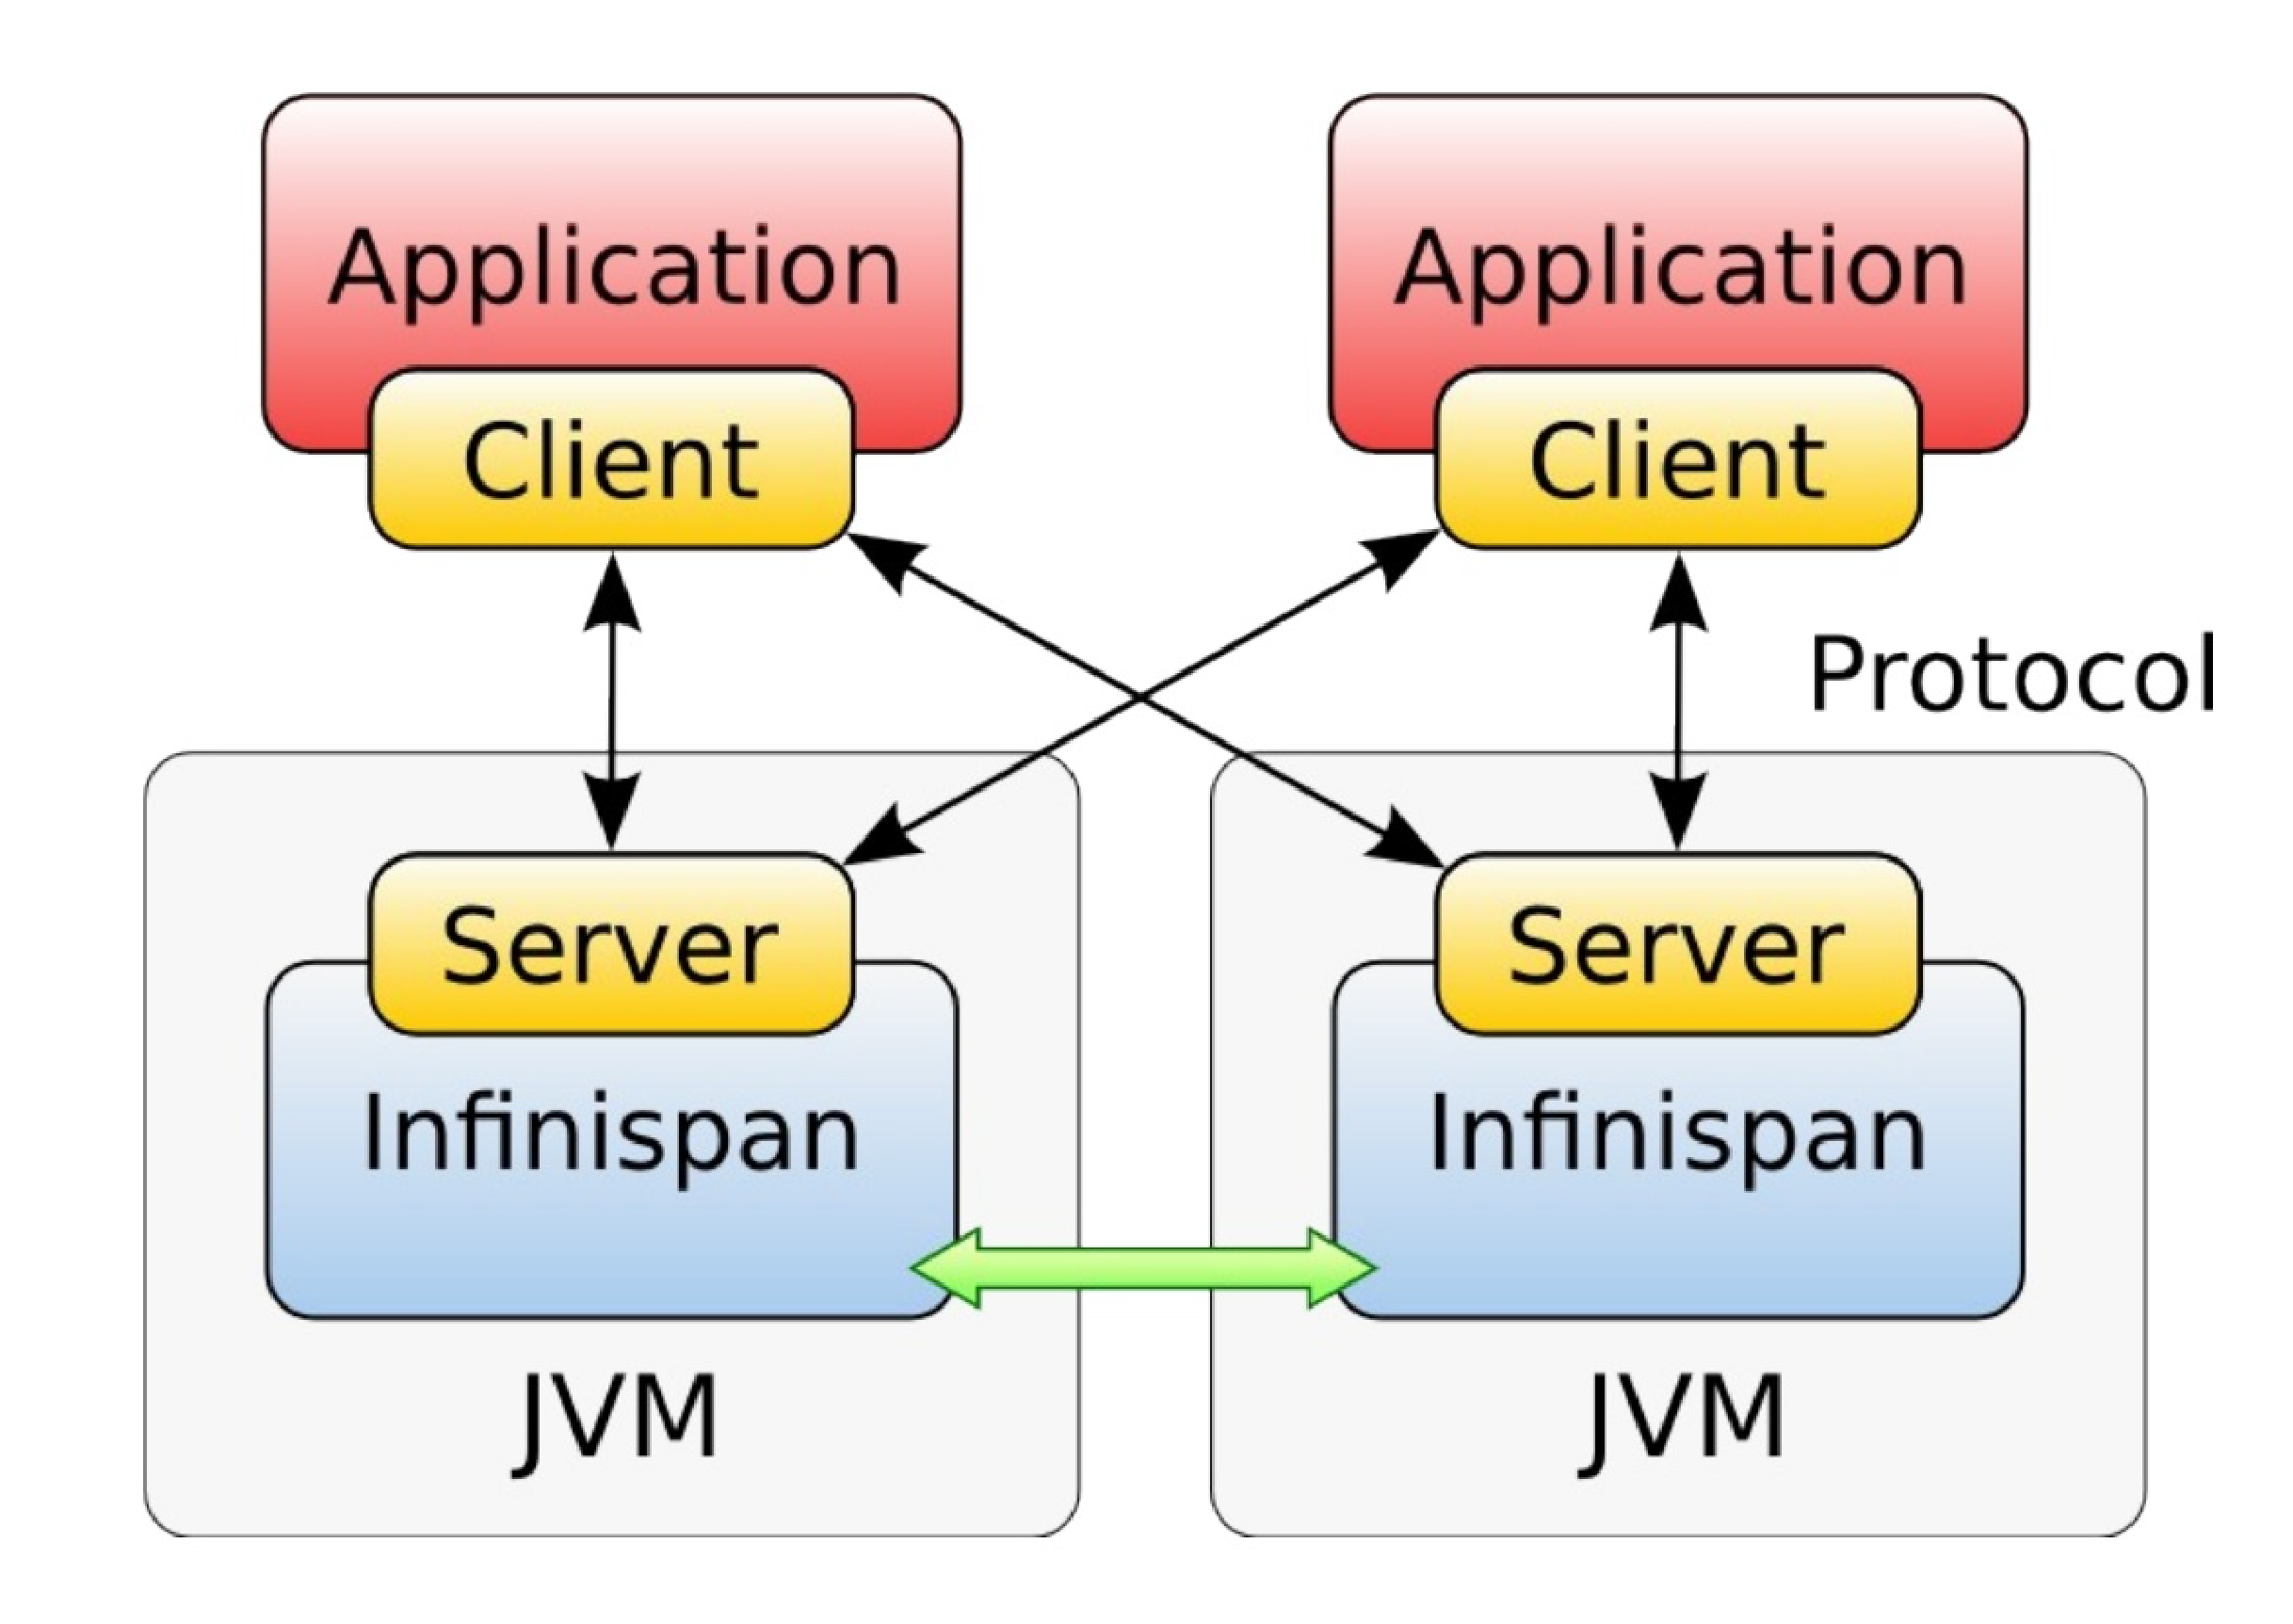
\includegraphics[width=5cm]{./img/ispn-cs.eps}
		\end{figure}
	\end{columns}
\end{frame}


\begin{frame}
	\frametitle{Remote protocols}
	\begin{columns}
	\column{0.5\textwidth}
		\begin{itemize}
			\item Hot Rod
				\begin{itemize}
					\item hashing and topology aware
					\item failover during topology changes
					\item smart request routing
				\end{itemize}
			\item Memcached
			\item REST
		\end{itemize}
	\column{0.5\textwidth}
		\begin{figure}
			%\centering
			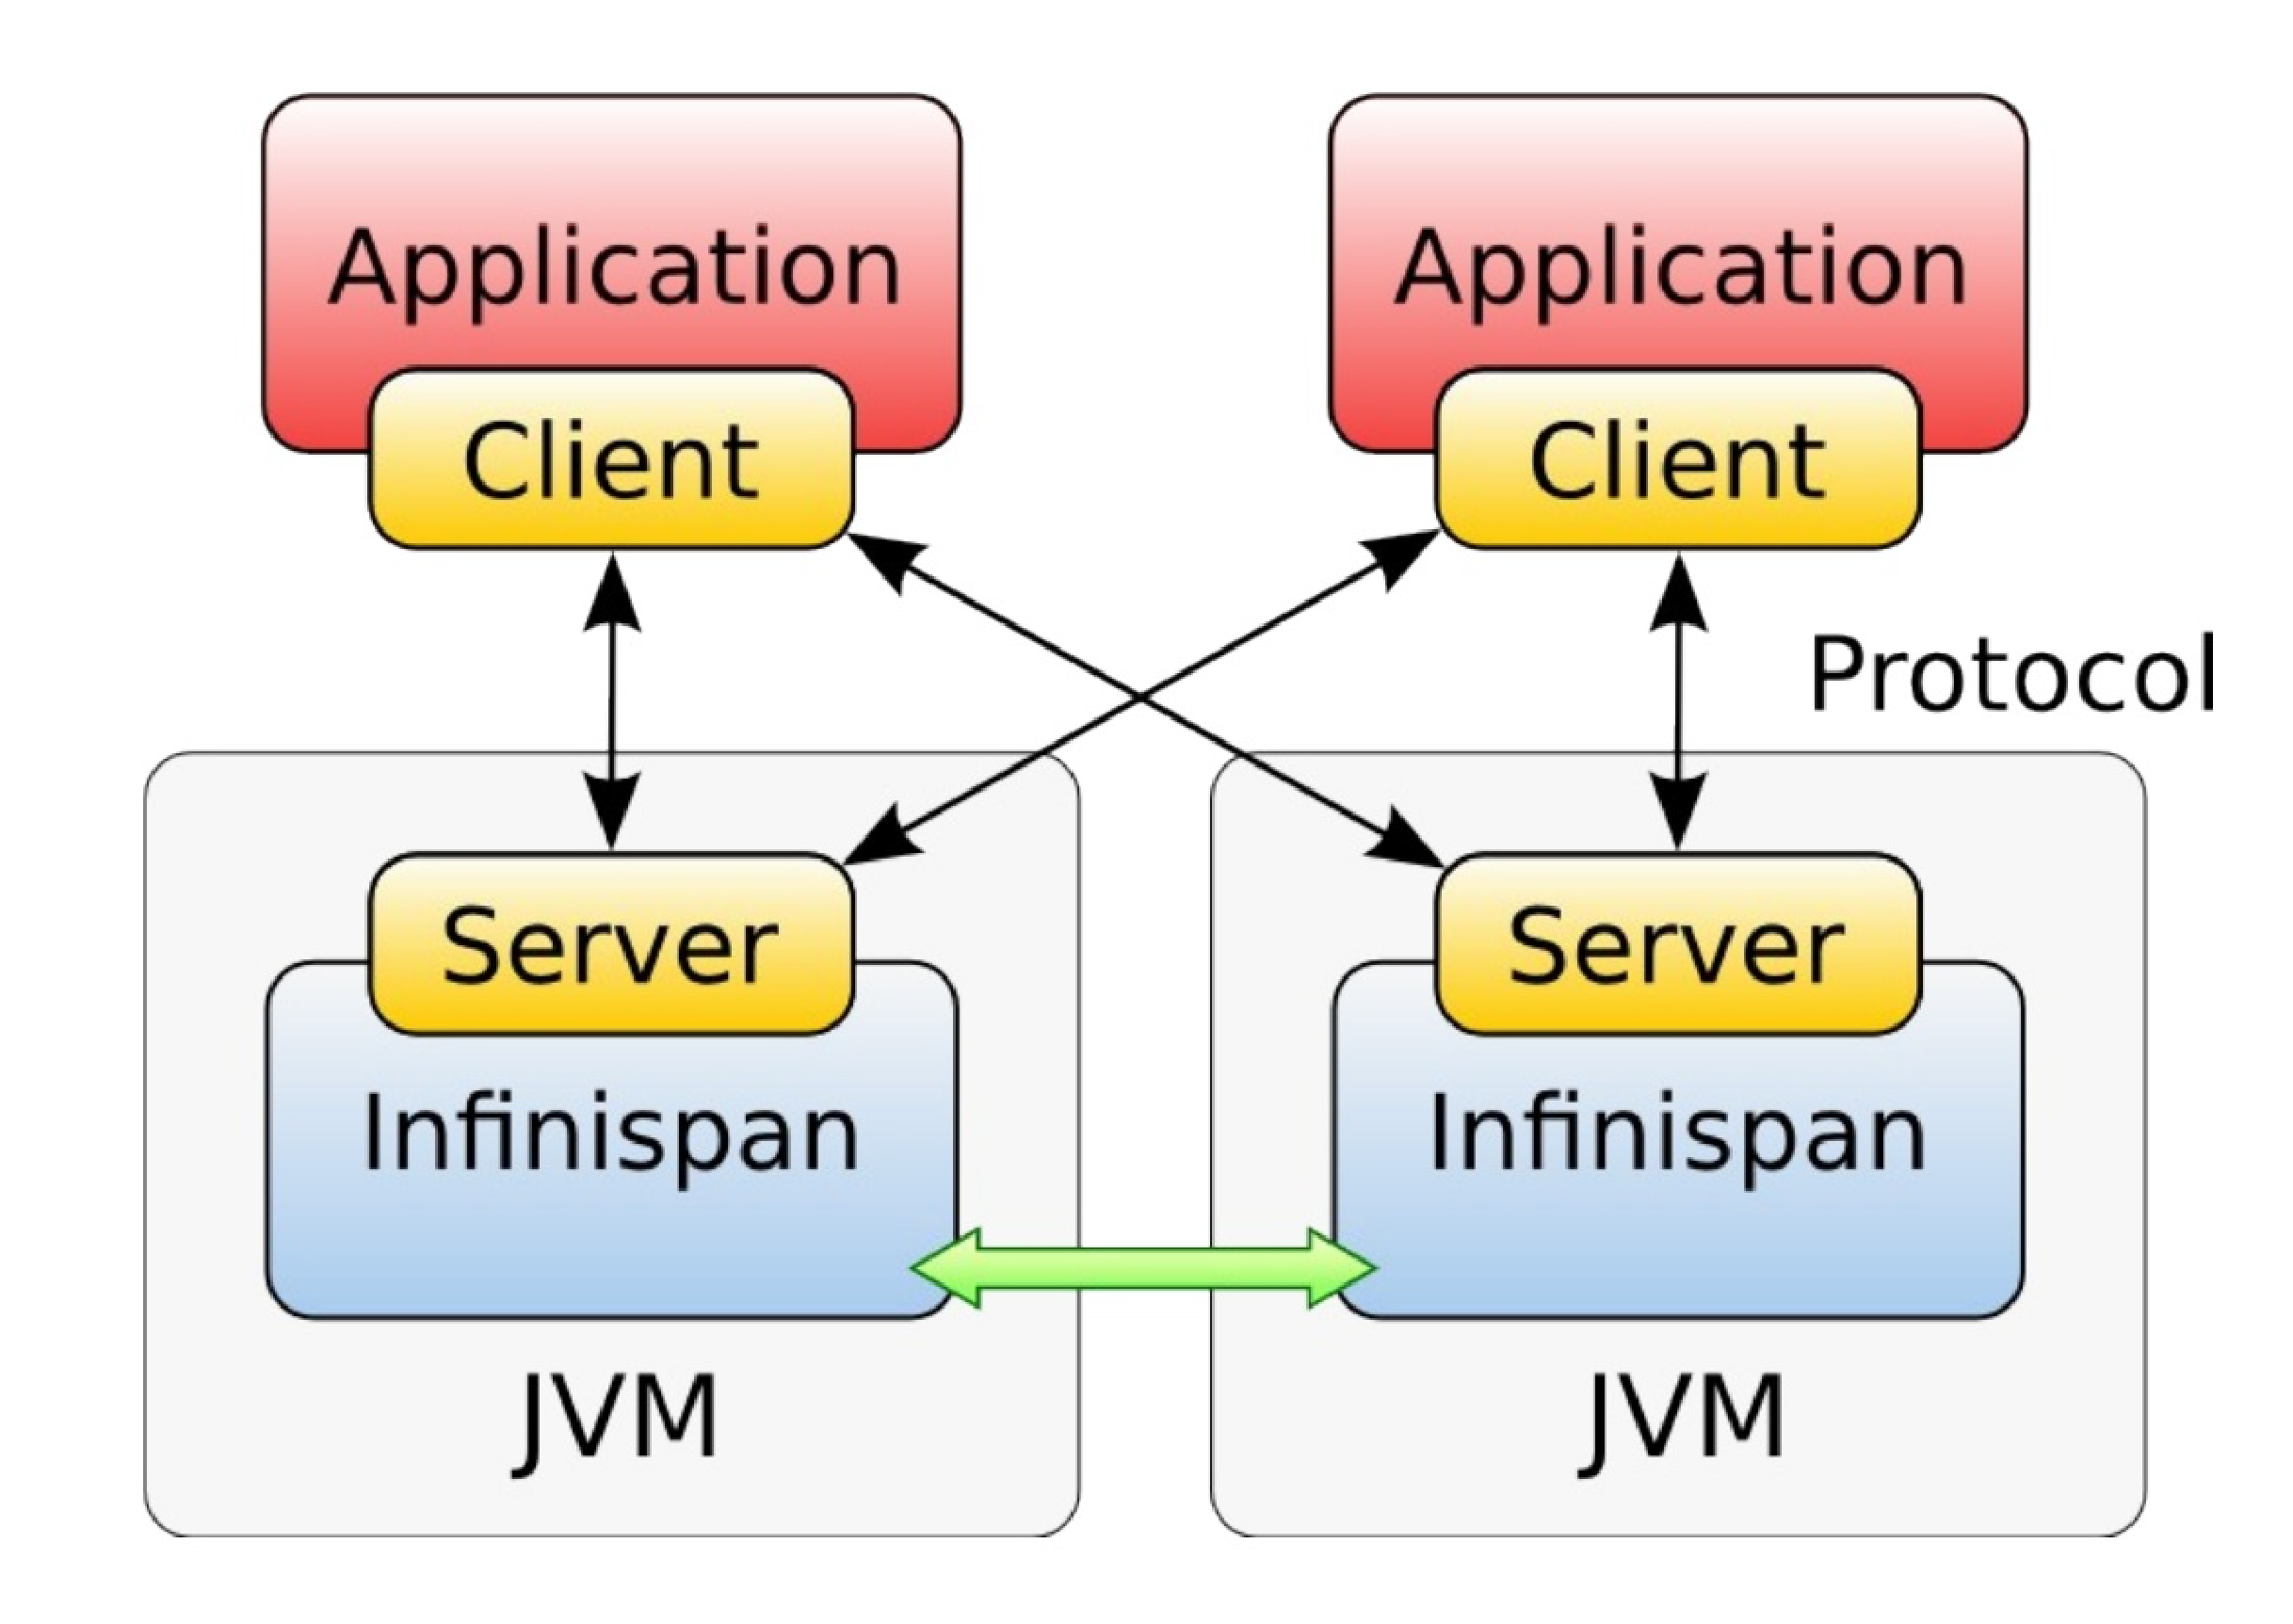
\includegraphics[width=5cm]{./img/ispn-cs.eps}
		\end{figure}
	\end{columns}
	
	\visible<2> {
	\scriptsize{
	\begin{table}
		\begin{tabular}{|c||c|c|c|c|c|}
		\hline
			& & & & & \\
		\textbf{Protocol} & \textbf{Format} & \textbf{Client libs} & \textbf{Clustered} & \textbf{Smart routing} & \textbf{Load balancing / Failover} \\
		 \hline
			& & & & & \\
		 \textbf{Hot Rod} & binary & Java, C++, C\# & yes & yes & dynamic \\
			& & & & & \\
		 \textbf{Memcached} & text & many & yes & no & only predefined server list \\
			& & & & & \\
		 \textbf{REST} & text & any HTTP client & yes & no & any HTTP load balancer \\
		 \hline
		\end{tabular}
	\end{table}
	}
	}
\end{frame}

\begin{frame}
  \frametitle{Hot Rod clients}
	Compatible with Java and non-Java platforms. Based on Protocol Buffers - Google's data interchange format.\\
	\vspace{0.5cm}
	Clients for
	\begin{itemize}
		\item Java
		\item C\#
		\item C++
		\item Python
		\item Ruby
	\end{itemize}
	Python and Ruby clients have only basic functionality.
\end{frame}

\begin{frame}[fragile]
	\frametitle{Commercial break: Protocol Buffers}
	\href{https://developers.google.com/protocol-buffers/}{\color{blue}\textbf{Protocol Buffers }} (protobuf) are language-neutral, platform-neutral, extensible mechanism for serializing 
	structured data developed by Google. \\ 
	\vspace{0.1cm}
	
	\begin{itemize}
		\item Supports C++, C\#, Go, Java, Python.
		\item You need to define data structure in protobuf file.
		\item In ISPN you can use also annotations in the your model.
	\end{itemize}
	
	Example of protobuf file:
	\begin{lstlisting}[style=Protobuf] 
	message Address {
    required string street = 1;
    required string postCode = 2;
	}

	 message Person {
    optional int32 id = 1;
    required string name = 2;
    required string surname = 3;
    optional Address address = 4;
    optional string license = 5;
    enum Gender {
      MALE = 0;
      FEMALE = 1;
    }                                                                                                                                                                                                                                         
	}                
	\end{lstlisting}
\end{frame}


\begin{frame}
	\frametitle{Cache stores}
	A way how to store cache content in some external (persistent) storage.\\

	\begin{columns}
	\column{0.6\textwidth}
	\visible<2,3> {
		Two modes:
		\begin{itemize}
			\item Synchronous (write-through)
			\item Asynchronous (write-behind)
		\end{itemize}
	}
	\visible<3> {
		Cache stores:
		\begin{itemize}
			\item Single file store and soft-index file store
			\item JDBC and JPA cache stores
			\item LevelDB cache store
			\item Cloud cache store
			\item Remote store
			\item Cassandra store
			\item \dots and others
		\end{itemize}
		Also possible to define custom cache store.
	}
	\column{0.4\textwidth}
		\begin{figure}
			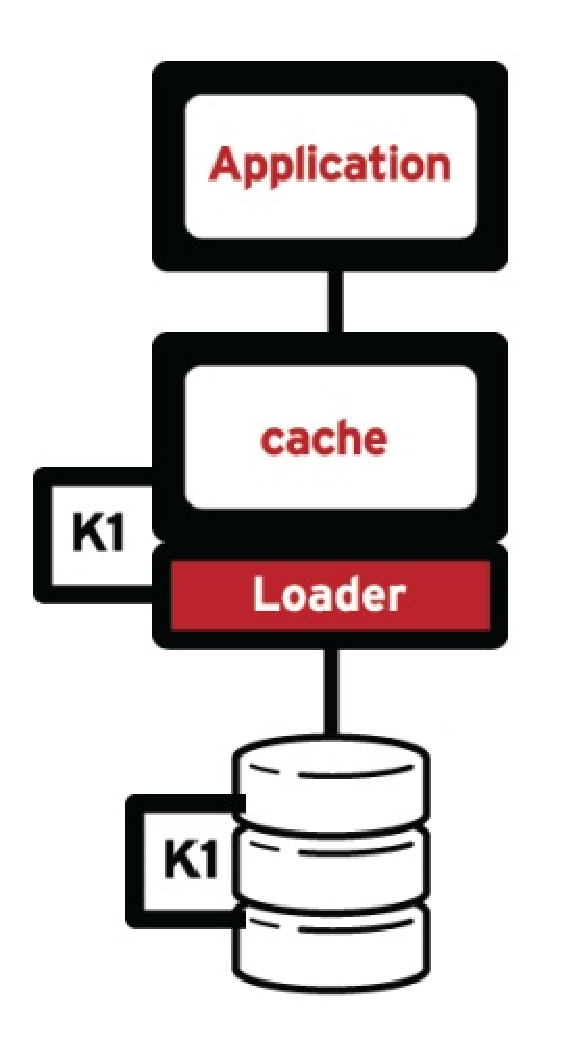
\includegraphics[width=3cm]{./img/cache_store.eps}
		\end{figure}
	\end{columns}
\end{frame}

\begin{frame}
	\frametitle{Transactions, consistency, locking and isolation}
	\begin{itemize}
		\item JTA-compliant transactions
		\pause
		\item Deadlock detection and recovery (e.g. when ISPN fails during commit phase of the transaction)
		\pause
		\item Data versioning
% 		\begin{itemize}
% 			\item Simple versioning
% 			\item Partition-aware versioning (vector locks)
% 			\item External versioning - used e.g. with Hibernate, where locks are provided by database
% 		\end{itemize}
		\pause
		\item Ensures consistency of data, consistency guarantee: 
		lock for key \texttt{K} is always, acquired on the same node of the cluster (key \textbf{primary owner}), regardless of where the transaction originates
	\end{itemize}
\end{frame}

\begin{frame}
	\frametitle{Transactions, consistency, locking and isolation (cont.)}
	\begin{itemize}
		\item \textbf{Pessimistic} and \textbf{optimistic} locking available
		\begin{itemize}
		\pause
		\item Pessimistic locking: resource is locked all the time during the transaction (in ISPN when resource is changed, read is still possible).
		\pause
		\item Optimistic locking: state of the resource is saved at the beginning of the transaction (prepare phase) and other transactions ca access the resource. During commit phase of the resource 
		is read again and if changed (write skew), transaction is rolled back.
		\end{itemize}
		\pause
		\item Isolation - how/when the changes made by one operation become visible to other. \textbf{Read committed} and \textbf{repeatable read} isolation levels.
			\begin{enumerate}
				\pause
				\item \color{MyDarkGreen}Thread1: tx.begin()
				\pause
				\item Thread1: cache.get(k) returns v
				\pause
				\item \color{magenta}Thread2: tx.begin()
				\pause
				\item Thread2: cache.get(k) returns v
				\pause
				\item Thread2: cache.put(k, v2)
				\pause
				\item Thread2: tx.commit()
				\pause
				\item \color{MyDarkGreen}Thread1: cache.get(k)
				\pause
			\end{enumerate}
			With \texttt{REPEATABLE\_READ}, step 7 will still return \texttt{v}, while with \texttt{READ\_COMMITTED} step 7 will return \texttt{v2}.
	\end{itemize}
\end{frame}

\begin{frame}
	\frametitle{Querying}
	\begin{itemize}
		\item Support for indexing and searching of objects stored in the cache.
		\pause
		\item Search for data using data attributes instead of keys.
		\pause
		\item Uses Hibernate Search and Apache Lucene to index and search objects.
		\pause
		\item Queries can be constructed using ISPN fluent DSL API, Hibernate Search Query DSL or directly Lucene query API.
		\pause
		\item Needs some data schema (protobuf file or annotations).
		\pause
		\item Combine queries and aggregation functions (but doesn't support joins).
		\pause
		\item Sort, filter, and paginate query results.
		\pause
		\item Support for index or non-indexed queries.
	\end{itemize}
\end{frame}

\begin{frame}[fragile]
	\frametitle{Querying: example}
	\begin{lstlisting}[style=Java]
  !@Indexed!
  public class Person {
    !@Field!(store = Store.YES, analyze = Analyze.NO)
    String name;

    !@Field!(store = Store.YES, analyze = Analyze.NO, indexNullAs = Field.DEFAULT_NULL_TOKEN)
    String surname;

    public Person(String name, String surname) {
      this.name = name;
      this.surname = surname;
    }
	}
	\end{lstlisting}
\end{frame}

\begin{frame}[fragile]
% 	\frametitle{Querying: example (cont.)}
% 	\vspace{-0.4cm}
	\begin{lstlisting}[style=Java]
	public class InfinispanQuery {
    public static void main(String[] args) {
      ConfigurationBuilder b = new ConfigurationBuilder();
      b.indexing().index(Index.ALL).addProperty("default.directory_provider", "ram").addProperty("lucene_version", "LUCENE_CURRENT");
      DefaultCacheManager cm = new DefaultCacheManager(builder.build());
      Cache<String, Person> cache = cm.getCache();
      cache.put("person1", new Person("Will", "Shakespeare"));
      // Obtain a query factory for the cache
      QueryFactory<?> queryFactory = Search.getQueryFactory(cache);
      // Construct a query
      Query query = queryFactory.from(Person.class).having("name").eq("Will").toBuilder().build();
      // Execute the query
      List<Person> matches = query.list();
      matches.forEach(person -> System.out.printf("Match: %s", person));
      cacheManager.stop();
   }
	}
	\end{lstlisting}
\end{frame}


\begin{frame}
	\frametitle{Security}
	\begin{itemize}
	 \item Role based access control
	 \pause
	 \item User authentication
	 \pause
	 \item Node authentication and authorization
	 \pause
	 \item Encryption of communication
	 \pause
	 \item Audit logging
	 \pause
	 \item Integration with LDAP and/or Kerberos server (includes Active Directory)
	\end{itemize}
\end{frame}


\begin{frame}
  \frametitle{Some other features - brief and selective list}
  \begin{itemize}
		\item Data eviction and expiration
		\pause
		\item Full JSR-107 support (Java Temporary Caching API)
		\pause
		\item CDI support
		\pause
		\item Remote events
		\pause
		\item Client near cache
		\pause
		\item Rolling upgrades
		\pause
		\item Cross data center replication (also Hot Rod clients support failover to another data center)
		\pause
		\item Command line interface
		\pause
		\item Distributed executors
  \end{itemize}
\end{frame}


\begin{frame}
	\frametitle{Recently implemented features: Infinispan 8}
	\begin{figure}
		\centering
		
\includegraphics[width=5cm]{./img/infinispan8.eps}
	\end{figure}
  \begin{itemize}
    \item Functional API
		\pause
		\item Distributed streams
		\pause
		\item Continuous querying, grouping and aggregation
		\pause
		\item New management console
		\pause
		\item Integration with Apache Spark and Hadoop
		\item \dots and more
  \end{itemize}
\end{frame}

\begin{frame}
	\frametitle{Integration with other frameworks}
	\begin{itemize}
		\pause
		\item Hibernate
		\begin{itemize}
			\item 2-nd level cache
		\end{itemize}
		\pause
		\item Lucene directory
		\begin{itemize}
		 \item In-memory Lucene index 
		\end{itemize}
		\pause
		\item Apache Camel
		\begin{itemize}
		 \item Infinispan component for Camel
		\end{itemize}
		\pause
		\item Hadoop
		\begin{itemize}
			\item In-memory data source for Hadoop cluster
		\end{itemize}
		\pause
		\item Apache Spark
		\begin{itemize}
			\item Data source for Spark map-reduce jobs
		\end{itemize}
	\end{itemize}
\end{frame}

\begin{frame}
	\frametitle{Summary}
	\begin{itemize}
		\pause
		\item Amount and structure of the data has changed rapidly during past couple of years.
		\pause
		\item Cloud applications and Big/Fast data require new approaches and tools, data grids are important building blocks of such solutions.
		\pause
		\item Infinispan is mature and feature rich data grid solution, which integrates well with other frameworks and can be used as backbone for new 
	 generation of enterprise applications.
	\end{itemize}
\end{frame}

\begin{frame}
	\frametitle{Materials from this course}
	\scriptsize{
	\begin{itemize}
		\item This presentation: \color{blue}\url{https://github.com/vjuranek/presentations/tree/master/CTU_Prague2016}\color{black}
		\item ISPN embedded tutorial (The Weather App): \color{blue}\url{http://infinispan.org/tutorials/embedded}\color{black}
		\item GitHub repo: \color{blue}\url{https://github.com/infinispan/infinispan-embedded-tutorial}\color{black}
		\item ISPN simple tutorials: \color{blue}\url{https://github.com/infinispan/infinispan-simple-tutorials}\color{black}
		\item ISPN qickstarts (simple applications) at the bottom of the page: \color{blue}\url{http://infinispan.org/tutorials}\color{black}
		\item Some more ISPN snippets: \color{blue}\url{https://github.com/vjuranek/infinispan-snippets}\color{black}
	\end{itemize}
	}
	\vspace{0.5cm}
	Infinispan downloads:
	\scriptsize{
	\begin{itemize}
		\item Main ISPN download page: \color{blue}\url{http://infinispan.org/download/}\color{black}
		\item If you want to play with ISPN in Docker: \color{blue}\url{https://hub.docker.com/r/jboss/infinispan-server/}\color{black}
	\end{itemize}
	}
\end{frame}

\begin{frame}
	\frametitle{Further study materials}
	\begin{itemize}
		\item \color{blue}\href{http://infinispan.org/documentation/}{Infinispan documentation}
		\item \href{https://jcp.org/en/jsr/detail?id=107}{JSR 107: JCACHE - Java Temporary Caching API}\color{black}
		\item M. Surtani, F. Marchioni, Infinispan Data Grid Platform,  Packt Publishing, 2012
		\item W. dos Santos, Infinispan Data Grid Platform Definitive Guide, Packt Publishing, 2015
		\item M. Kleppmann, Designing Data-Intensive Applications, O'Reilly Media, Inc., 2016
		\vspace{0.5cm}
		\item  B. Burke, A. Rubinger, Enterprise JavaBeans 3.1, 6th Edition,  O'Reilly Media, Inc., 2010
		\vspace{0.5cm}
		\color{blue}
		\item \href{https://www.coursera.org/course/cloudcomputing}{Coursera: Cloud Computing Concepts}
		\item \href{https://www.coursera.org/course/cloudcomputing2}{Coursera: Cloud Computing Concepts: Part 2}
		\item \href{https://www.coursera.org/course/cloudapplications}{Coursera: Cloud Computing Applications}
	\end{itemize}
\end{frame}

\begin{frame}
	\frametitle{Question?}
	\begin{figure}
		\centering
		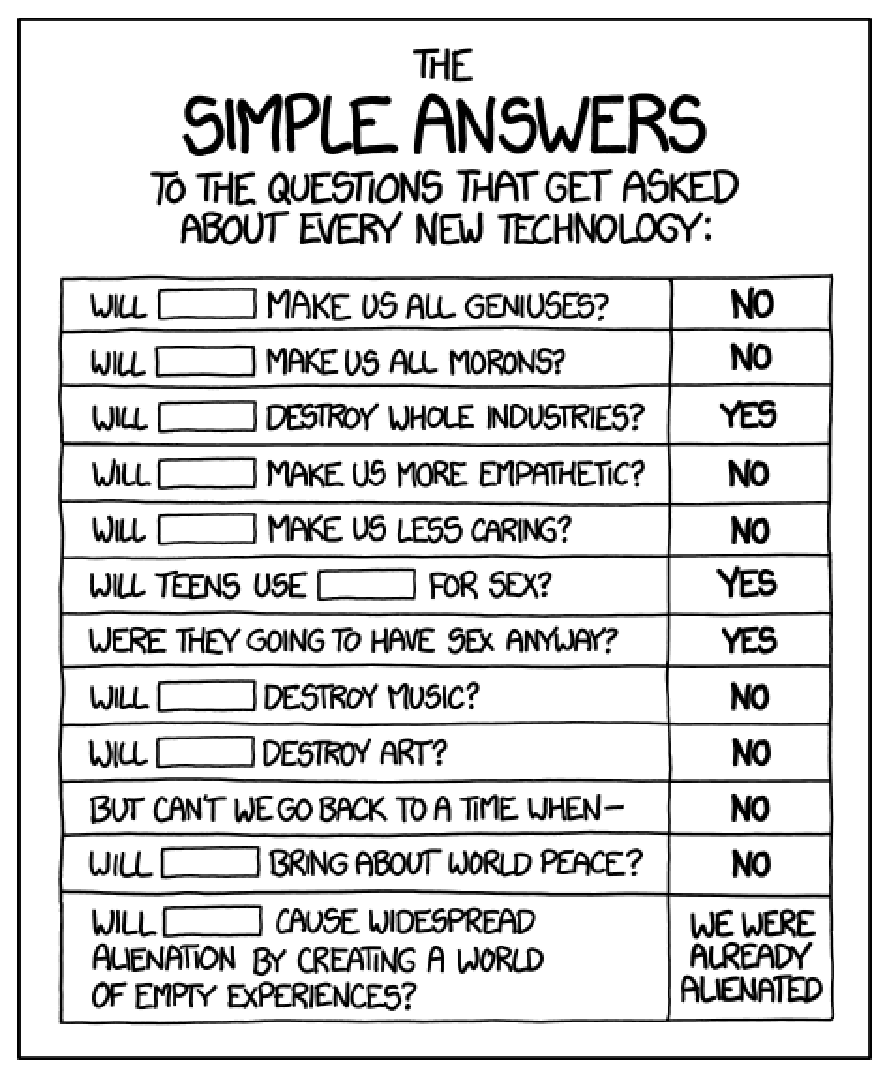
\includegraphics[width=6cm]{./img/simple_answers.eps}
		\caption{\tiny{Source: \url{https://xkcd.com/1289/}}}
	\end{figure}
\end{frame}

\begin{frame}
	\centering
	\huge{\color{blue}{\url{http://infinispan.org/}}} \\
	\vspace{1cm}
	\huge{\textbf{Thank you for your attention!}} \\
	\vspace{1cm}
\end{frame}



\end{document}